\chapter{Kategorisierung von Bewegungsdaten mittels deterministischer Algorithmen}
\label{chapter2}
Nach den einführenden Bemerkungen in \autoref{chapter1} werden nun die grundliegenden Punkte beschrieben,
die bei der Umsetzung eines Kategorisierungssystems für \ac{TSD} zu beachten sind.
Anschließend wird das eingesetzte Vorgehen erläutert und an einem Beispiel veranschaulicht.
Ein Einlick in verwandte Arbeiten (\autoref{chapter2-RelatedWork}) vertieft das Verständnis weiter.
Abschließend wird auf zu beachtende Besonderheiten des Kinect-Datensatzes eingegangen.


\section{Problembeschreibung}
\label{chapter2-Problembeschreibung}
Beim vorliegenden Kinect-Datensatz sind zwei wesentliche Punkte zu beachten.
Zum einen handelt es sich um einen eine große Datenmenge.
Die einzelnen Datenpunkte müssen daher automatisiert bearbeitet werden.
Ziel der Verarbeitung ist es möglichst sinnvolle \emph{Cluster} zu erhalten.
Um die Gemeinsamkeiten zweier Datenpunkte zu berechnen,
wird eine geeignete Vergleichsfunktion benötigt.
Die Wahl dieser Funktion ist wichtig für den Erfolg des \emph{Clusterings} \citep{warren_liao_clustering_2005}.
Zu beachten ist zudem, dass die Bewegungsaufnahmen durch \emph{\ac{TSD}} beschrieben werden.
Bei diesem Datentyp handelt es sich um geordnete Sequenzen von Datenpunkten,
die über eine gewisse Zeit hinweg aufgenommen werden.
Oft in regelmäßigen Abständen \citep{ali_clustering_2019}.
Werden hier herkömmliche Distanzmetriken, wie die Euklidische-Distanz verwendet
kann dies zu Problemen führen und die Aussagekraft des Vergleichs verringern.
Es kann vorkommen, dass verschiedene Personen die gleiche Bewegung unterschiedlich schnell ausführen.
Gegebenenfalls weisen die Datenreihen bei der gleichen Bewegung daher sogar eine unterschiedliche Anzahl an Frames auf.
\autoref{fig:MetricComparison} zeigt ein exemplarisches Szenario.
Die Kurven weisen ähnliche Segmente auf.
Sie sind allerdings unterschiedlich lang und die Ähnlichkeiten treten zu unterschiedlichen Zeitpunkten auf.
Mit der bekannten euklidischen Distanz ist das Ergebnis hier nicht aussagekräftig
und der letzte Punkt der Reihe kann gar nicht zugordnet werden.
Um dieses Problem zu lösen ist eine elastische Metrik nötig,
die besser mit zeitlichen Verschiebungen umgehen kann \citep{aghabozorgi_time-series_2015}.

\begin{figure}[ht]
    \begin{center}
    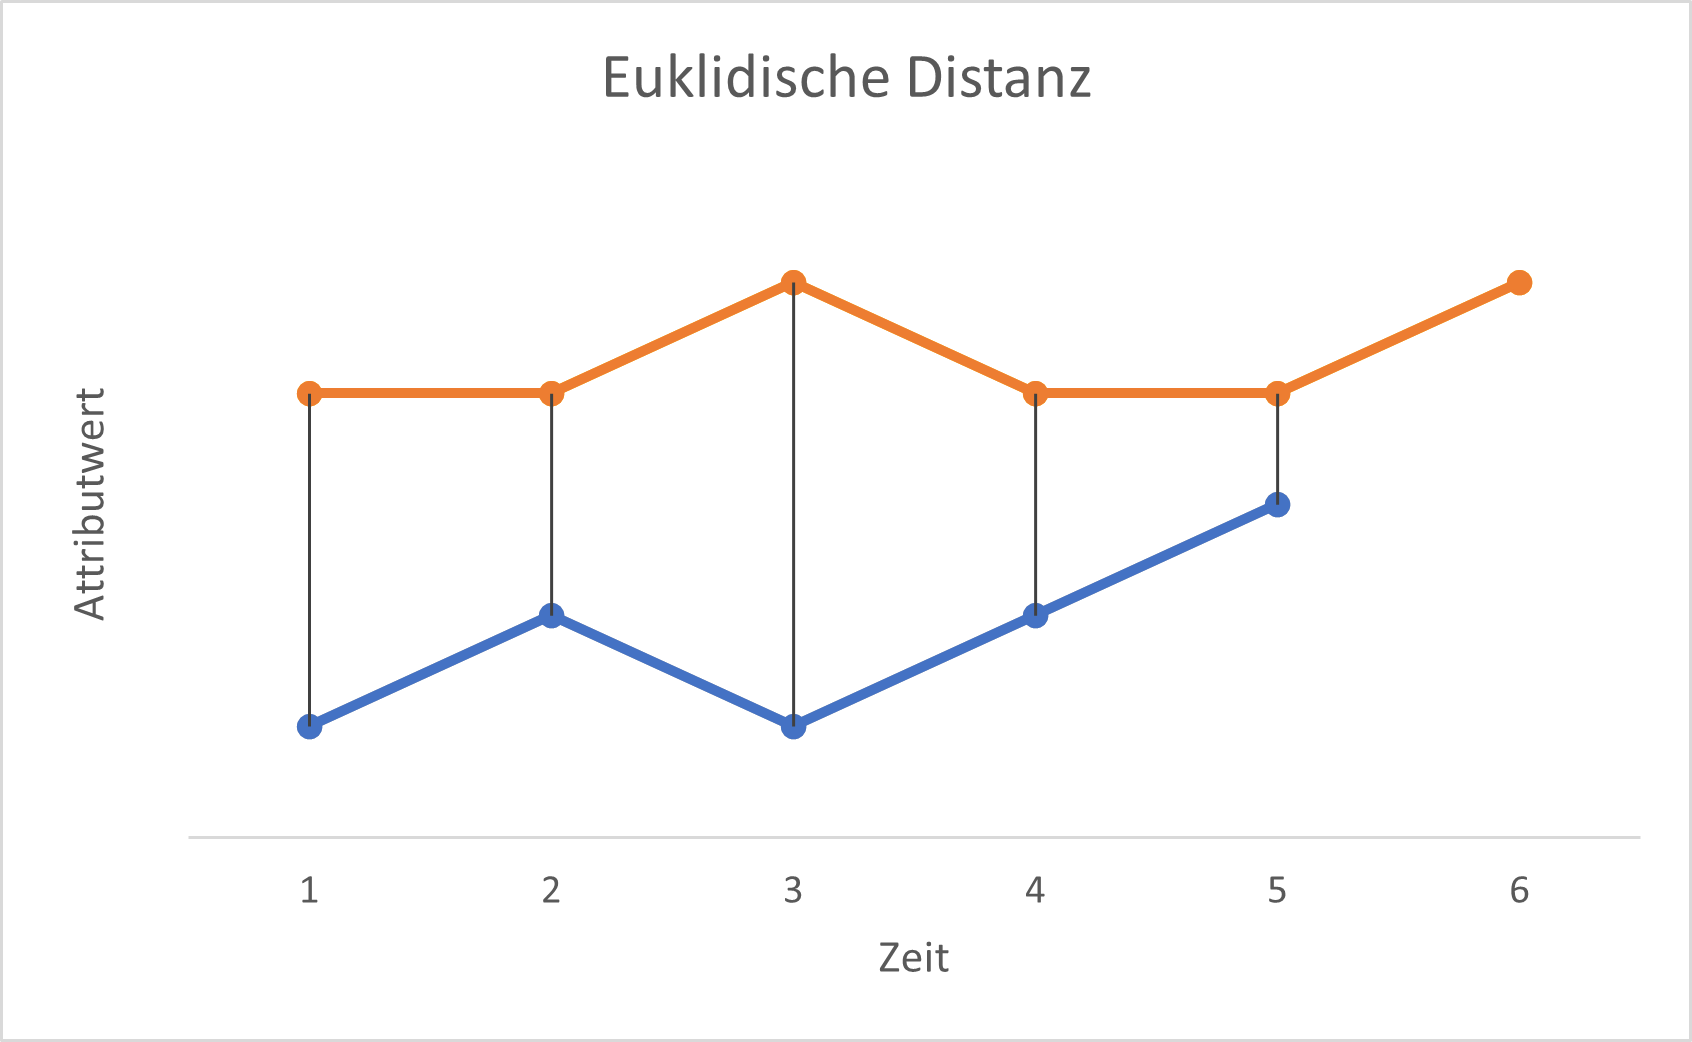
\includegraphics[width=0.45\textwidth]{EuclidianMetric.png}
    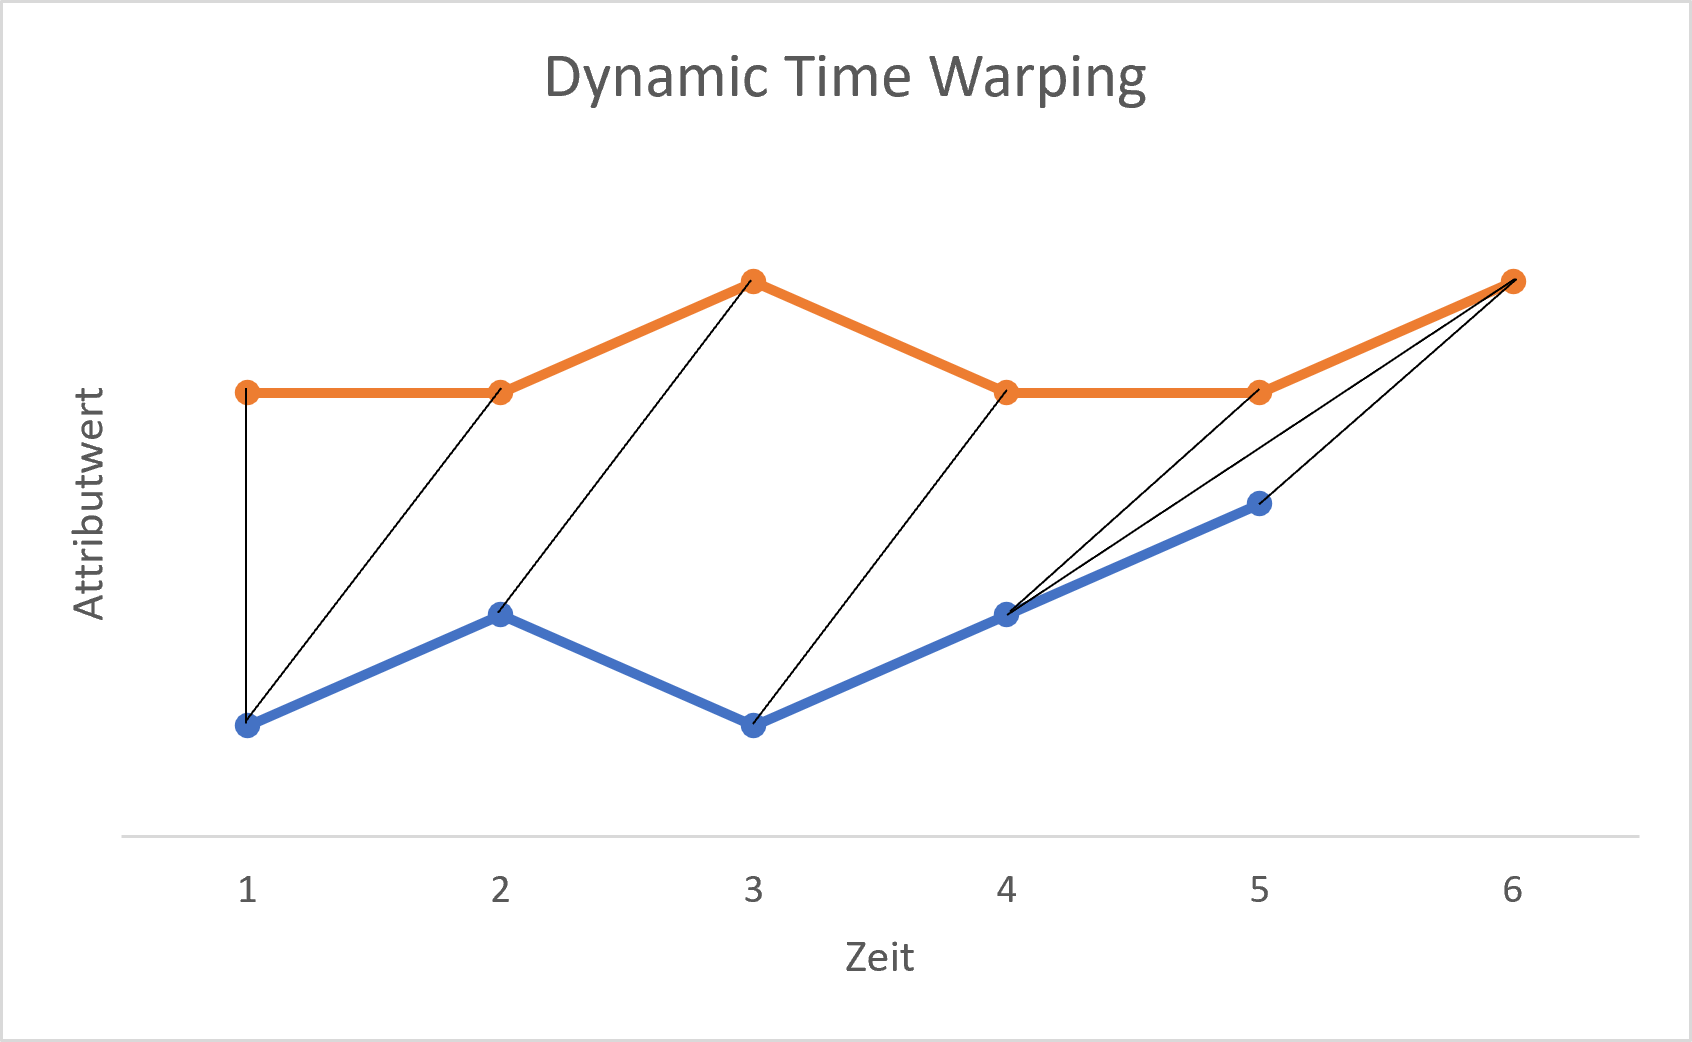
\includegraphics[width=0.45\textwidth]{DTWMetric.png}
    \end{center}
    \caption{Zuorndung der Messpunkte zweier Datenreihen.}
    \label{fig:MetricComparison}
\end{figure}

Das Clustering soll mithilfe von \emph{hierarchischem Clustern} durchgeführt werden,
welches in \autoref{chapter2-Clustering} beschrieben wird.
Als geeignete Distanz-Metrik wird dabei \emph{\ac{DTW}} verwendet (\autoref{chapter2-DTW}).
Hier ist eine Mehrfachzuordnung von Punkten möglich.
Diese können so verbunden werden, dass die Kosten minimal sind.
Dies erlaubt eine Zuordnung ähnlicher Muster in den Daten auch wenn sie zeitlich verschoben sind.

\section{Hierarchisches Time-Series Clustering}
\label{chapter2-Clustering}
\emph{Clustering} kann genutzt werden, um große Datensätze zu kategorisieren,
wenn keine Informationen zu den Kategorien vorliegen \citep{aghabozorgi_time-series_2015}.
Ziel ist es, eine Struktur in den vorliegenden Daten zu finden,
indem Elemente anhand eines festgelegten Vorgehens in homogene Gruppen einsortiert werden.
Dabei sollen die Unterschiede bei Elementen der gleichen Gruppe möglichst gering
und bei Elementen verschiedener Gruppen möglichst groß sein \citep{aghabozorgi_time-series_2015, warren_liao_clustering_2005}.
Bei \emph{n} Datenpunkten erzeugt ein \emph{Clustering} \emph{k} Partitionen des Datensatzes.
Jede Partition entspricht dabei einem \emph{Cluster}, dass mindestens ein Objekt enthält.
Zum \emph{Clustering} sind besonders die Wahl des Clustering-Algorithmus
und der Methode zur Bestimmung der Ähnlichkeit von zwei Datenreihen von Bedeutung \citep{warren_liao_clustering_2005}.
Letzteres wird \ac{DTW} gelöst und in \autoref{chapter2-DTW} beschrieben.
Als Clustering-Vorgehen kann das sogenannte \emph{hierarchical Clustering} genutzt werden.
Dieses funktioniert, indem Datenobjekte in einen Baum von Clustern eingeteilt werden.
Bei agglomerativen Vorgehen wird ein \emph{bottom-up} Ansatz verfolgt.
Jedes Objekt ist daher zunächst ein eigenes Cluster.
Dann werden schrittweise Cluster zusammengeführt,
bis alle Objekte im selben Cluster sind, oder eine Terminierungsbedingung erfüllt ist \citep{warren_liao_clustering_2005}.

Im Fall des Kinect-Datensatzes liegen die Daten als \ac{TSD} vor.
\ac{TSD} zu kategorisieren findet in vielen wissenschaftlichen Gebieten Anwendung, um Muster zu finden.
Sie erlauben es wichtige Informationen aus großen Datensätzen zu extrahieren.
\ac{TSD} sind dynamische Daten, weil sich die Attributwerte mit der Zeit verändern.
Diese Sammlungen von Werten können aber auch als ein einziges Objekt betrachtet werden.
Das Kategorisieren von derartigen Objekten kann bei der Detektion relevanter Muster helfen \citep{aghabozorgi_time-series_2015}.
Die meisten bestehenden Cluster-Algorithmen können auf diesen Datentypen zugeschnitten werden.
So auch das hierarchische Clustering.
Der größte Unterschied ist wie bereits erwähnt, dass die Distanz-/ Ähnlichkeitsmetrik angepasst werden muss,
um sinnvoll bei \ac{TSD} genutzt werden zu können.
Ein Vorteil ist, dass hierarchisches Clustern bei der Verwendung von \ac{DTW}
nicht auf Datenreihen der gleichen Länge beschränkt ist \citep{warren_liao_clustering_2005}.


\section{Dynamic Time Warping Algorithmus}
\label{chapter2-DTW}
Der \emph{\ac{DTW} Algorithmus} kann als Distanz-Metrik beim hierarchischen Clustern genutzt werden.
Hier sind \emph{one-to-many} oder \emph{one-to-none} Beziehungen zwischen Datenpunkten möglich.
Man bezeichnet das Vorgehen daher auch als eine \emph{elastische Metrik}.
Sie kann gut mit zeitlichen Verschiebungen und unterschiedlich langen Datenreihen umgehen \citep{aghabozorgi_time-series_2015}.

In der Literatur findet man viele Erläuterungen des \ac{DTW}-Algorithmus.
Beispielsweise in \citet{mohammadzade_dynamic_2021}, \citet{warren_liao_clustering_2005},
\citet{aghabozorgi_time-series_2015} oder \citet{yu_dynamic_2019}.
Im Folgenden soll der Algorithmus ebenfalls erläutert werden.
Das Ziel ist die Zuordnung verschiedener Signale,
die im Verlauf der Zeit ähnliche Muster aufweisen.
Diese Muster treten zu unterschiedlichen Zeiten oder in unterschiedlichen Raten auf.
Um die Zuweisung zueinander zu erreichen muss jedes Signal gegebenenfalls lokal gestreckt oder gestaucht werden.
Durch \emph{dynamisches Programmieren} kann eine Korrespondenz zwischen den Zeitindizes zweier Signale gefunden werden,
sodass die Summe der Distanzen zwischen den beiden Signalen minimal ist \citep{mohammadzade_dynamic_2021}.

Seien \emph{Q = $q_{1}, q_{2}, ... , q_{i}, ... , q_{n}$} und \emph{R = $r_{1}, r_{2}, ... , r_{j}, ... , r_{n}$}
zwei Signale die durch \ac{DTW} ausgerichtet werden sollen, sodass die Differenz zwischen ihnen minimal ist.
Dafür wird eine \emph{n x m} Matrix \emph{M} gebildet, wobei das Element \emph{(i, j)} die Distanz \emph{$d(q_{i}, r_{j})$}
zwischen zwei Punkten \emph{$q_{i}$} und \emph{$r_{j}$} enthält.
Hierfür wird im Normalfall die euklidische Distanz genutzt \citep{warren_liao_clustering_2005}.
In der Zelle \emph{(0, 0)} enthält die Matrix den Wert 0
und für die übrigen Zellen der Spalte und Zeile 0 wird jeweils der Wert unendlich angenommen.
Das Verfahren kann auf einfache Weise auf mehrdimensionale \ac{TSD} angepasst werden.
In diesem Fall sind die zu minimierenden Kosten die Summe
der Distanzen zwischen den korrespondierenden Werten der beiden Datenreihen \citep{mohammadzade_dynamic_2021}.
Ein \emph{Warping Pfad} \emph{W = $w_{1}, w_{2}, ... , w_{k}, ... , w_{K}$} in dem \emph{$max(m, n) \le K \le m + n - 1$} gilt,
ist eine Reihe von Matrixelementen die drei Bedingungen erfüllen:
\begin{itemize}
    \item Grenzbedingungen
    \item Kontinuität
    \item Monotonität
\end{itemize}
Die Grenzbedingungen fordern, dass die Startzelle des Warping Pfads in der Matrix eine andere ist als die Zielzelle.
Dabei gilt: \emph{$w_{1}$ = (m, n)} und \emph{$w_{k}$ = (0, 0)}.
Aufgrund der Kontinuität sind nur Schritte in angrenzende Zellen erlaubt.
Die Monotonitätsbedingung zwingt den Warping Pfad dazu, sich monoton in der Zeit zu bewegen.

Mit Hilfe von dynamischer Programmierung können die Matrixeinträge von \emph{$M_{(0, 0)}$} ausgehend berechnet werden,
indem wiederholt die folgende Gleichung ausgewertet wird.
\emph{$ M_{(i, j)} = d(q_{i}, r_{j}) + min $ \{$M_{(i - 1, j - 1)}, M_{(i - 1, j)}, M_{(i, j - 1)} $\}}
Sie definiert den kumulativen Abstand als die Summe aus dem Abstand des aktuellen Elementes
und dem Minimum der kumulativen Abstände der benachbarten Elemente \citep{warren_liao_clustering_2005}.
Der Pfad mit der minimalen Distanz ist von Bedeutung.
Er kann mit \emph{$d_{DTW} = min(\frac{\sum_{k = 1}^{K}w_{k}}{K})$} berechnet werden.


\section{Veranschaulichendes Beispiel}
\label{chapter2-Example}
Zur Veranschaulichung soll nun das Vorgehen anhand von vier Datenreihen durchgeführt werden.
Seien \emph{$R_{1}$ = (0, 1, 1, 2, 2, 1, 1)}, \emph{$R_{2}$ = (0, 1, 1, 1, 2, 2, 1, 1)}, \emph{$R_{3}$ = (1, 1, 0, 1, 2, 2, 1, 1)}
und \emph{$R_{4}$ = (2, 2, 1, 2, 2, 2)} gegeben.
Die Kosten können berechnet werden, indem die Kostenmatrix aufgestellt und der Warping Pfad berechnet wird (\autoref{chapter2-DTW}).
Für die Berechnung der Kosten zwischen \emph{$R_{1}$} und \emph{$R_{2}$} ergibt sich beispielsweise folgende Matrix
mit hervorgehobenem Warping Pfad.
\begin{center}
    \begin{tabular}{ |c|c|c|c|c|c|c|c|c| } 
     \hline
     \textbf{0} & $\infty$ & $\infty$ & $\infty$ & $\infty$ & $\infty$ & $\infty$ & $\infty$ & $\infty$ \\
     \hline
     $\infty$ &\textbf{0} & 1 & 2 & 3 & 5 & 7 & 8 & 9 \\
     \hline
     $\infty$ & 1 & \textbf{0} & \textbf{0} & 0 & 1 & 2 & 2 & 2 \\
     \hline
     $\infty$ & 2 & 0 & 0 & \textbf{0} & 1 & 2 & 2 & 2 \\
     \hline
     $\infty$ & 4 & 1 & 1 & 1 & \textbf{0} & 0 & 1 & 2 \\
     \hline
     $\infty$ & 6 & 2 & 2 & 2 & 0 & \textbf{0} & 1 & 2 \\
     \hline
     $\infty$ & 7 & 2 & 2 & 2 & 1 & 1 & \textbf{0} & 0 \\
     \hline
     $\infty$ & 8 & 2 & 2 & 2 & 2 & 2 & 0 & \textbf{0} \\
     \hline
    \end{tabular}
\end{center}
Außerdem ergeben sich folgende gerundete Kosten zwischen den einzelnen Reihen: 
\begin{center}
    \begin{tabular}{ |c|c|c| } 
     \hline
     Reihen & Kosten \\
     \hline \hline
     $R_{1}$, $R_{2}$ & \textbf{0} \\
     \hline
     $R_{1}$, $R_{3}$ & 1.56 \\
     \hline
     $R_{1}$, $R_{4}$ & 2.88 \\
     \hline
     $R_{2}$, $R_{3}$ & 2.89 \\
     \hline
     $R_{3}$, $R_{4}$ & 2.67 \\
     \hline
    \end{tabular}
\end{center}
Da \emph{$R_{1}$} und \emph{$R_{2}$} zusammen die geringsten Kosten haben bilden sie das erste Cluster \emph{$C_{1}$}.
Um dessen Wertreihe zu erhalten werden die Attributwerte paarweise addiert und die Summe anschließend halbiert.
Dabei kann anhand des Warping Pfads abgelesen werden, welche Werte zusammengehören.
So ergibt sich \emph{$C_{1}$ = (0, 1, 1, 1, 2, 2, 1, 1)}.
Es sollte ein \emph{Threshold} definiert werden,
der angibt, ab wann die Kosten zu groß sind, um die beiden Datenreihen zu einem Cluster zusammenzuführen.
Ein sinnvoller Wert hängt dabei vom vorliegenden Datensatz ab.
Sei dieser Threshold im Folgenden \emph{t = 2}.
Nun werden die Schritte wiederholt, wobei \emph{$C_{1}$} als eine einzelne neue Datenreihe betrachtet wird.
Dabei ergeben sich folgende Kosten:
\begin{center}
    \begin{tabular}{ |c|c|c| } 
     \hline
     Reihen & Kosten \\
     \hline \hline
     $C_{1}$, $R_{3}$ & \textbf{1.56} \\
     \hline
     $C_{1}$, $R_{4}$ & 2.89 \\
     \hline
     $R_{3}$, $R_{4}$ & 2.67 \\
     \hline
    \end{tabular}
\end{center}
Nun haben \emph{$C_{1}$} und \emph{$R_{3}$} die geringsten Kombinationskosten.
Da die Kosten geringer sind als der Threshold kann ein neues Cluster gebildet werden.
Es ergibt sich \emph{$C_{2}$ = (0.5, 1, 0.5, 1, 2, 2, 1, 1)}.
Damit können die neuen Kosten berechnet werden:
\begin{center}
    \begin{tabular}{ |c|c|c| } 
     \hline
     Reihen & Kosten \\
     \hline \hline
     $C_{2}$, $R_{4}$ & \textbf{2.78} \\
     \hline
    \end{tabular}
\end{center}
Da die berechneten Kosten den zuvor definierten Threshold übersteigen wird kein neues Cluster mehr gebildet
und wir sind am Ende unserer Berechnungen angekommen.
\autoref{fig:Dendrogram} veranschaulicht die gebildeten Cluster.

\begin{figure}[ht]
    \begin{center}
    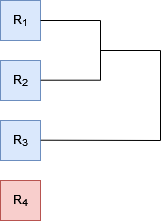
\includegraphics[width=0.25\textwidth]{dendrogram.png}
    \end{center}
    \caption{Graphische Veranschaulichung der gebildeten Cluster.}
    \label{fig:Dendrogram}
\end{figure}


\section{Related Work Analyse}
\label{chapter2-RelatedWork}
ToDo


\section{Einsatz im Kontext von Kinect-Bewegungsdaten}
\label{chapter2-Einsatz}
Wie bereits erwähnt handelt es sich bei den vorliegenden Daten um \ac{TSD}.
\citet{warren_liao_clustering_2005} und \citet{aghabozorgi_time-series_2015} weisen darauf hin,
dass besonders die verwendete Distanz-/ Ähnlichkeitsmetrik entscheidend ist,
um diesen Datentyp sinnvoll in Kategorien einteilen zu können.
Hierarchisches Clustering in Kombination mit \ac{DTW} scheint ein vielversprechender Ansatz zu sein.
Da die Daten in Textdateien vorliegen ist eine Komponente im System nötig,
die diese Informationen ausliest und in geeigneten Objekten der genutzten Programmiersprache abspeichert.
Besonders von Bedeutung ist zudem die Wahl geeigneter Attribute.
Die Daten enthalten viele Werte die mehr oder weniger interessant für die Kategorisierung sein können.
Die Laufwege oder Engagement-Werte sind beispielsweise relevanter als die Tatsache,
ob eine Person Brillenträger ist oder nicht.
Idealerweise sollte die Wahl der genutzten Attribute vom Nutzer der Anwendung definiert werden können.
So kann das Tool effektiv genutzt werden, um nach wiederkehrenden Abläufen in den Daten zu suchen.
Des weiteren stellt sich die Frage, ab wann keine weitere Clusterbildung mehr stattfinden soll.
Dazu muss ein geeigneter Threshold definiert werden.
Zudem ist die große Menge der Daten zu erwähnen.
\citet{aghabozorgi_time-series_2015} weist darauf hin,
dass \ac{DTW} weniger performant ist als herkömmliche Metriken wie die euklidische Distanz.
Gegebenenfalls müssen die Daten vor der Nutzung geeignet gefilter werden.
Diese Filterung soll allerdings nicht Bestandteil dieser Bachelorarbeit sein.